  	
  %-----------------------------------------------------------------%
  %   Architecture et explication détaillé de l'implémentation
  %-----------------------------------------------------------------%
  \chapter{Architecture du programme}
  
  \section{Lancement du programme}
  A été rajouté au programme des options de lancement, l'usage est disponible 
  
  \section{Carte de hauteur}
  
  Le programme utilise un \emph{quadtree} pour générer les différents niveaux de détail. 
  Ensuite une nouvelle hauteur est appliquée à ce point pour le déplacer. 
  Cependant, le \emph{quadtree} ne stocke pas la hauteur du sommet. Cette dernière
  est enregistrée dans une texture 2d et est envoyé à la carte graphique. 
  Chaque pixel de la texture représente donc une valeur codée sur un nombre flottant entre -1 et 1.
  La texture récupérée par la carte graphique, est plaquée sur le maillage de la sphère et la hauteur du sommet
  est déduite de l'interpolation des texels de la texture sur le maillage.
  %définir texel
  %définir interpolation ?
  
  
  \section{Système de rendu}
  Le programme est découpé en classes afin d'abstraire les appels à la bibliothèque OpenGL. La figure \ref{fig:uml_scene} représente le diagramme des classes qui forment l'abstraction principale du programme.
  Les classes relatives à la génération, l'affichage de la planète et l'utilisation du CDLOD sont strockés dans le dossier
  PlanetTech.
  
  \begin{figure}
  \centering
  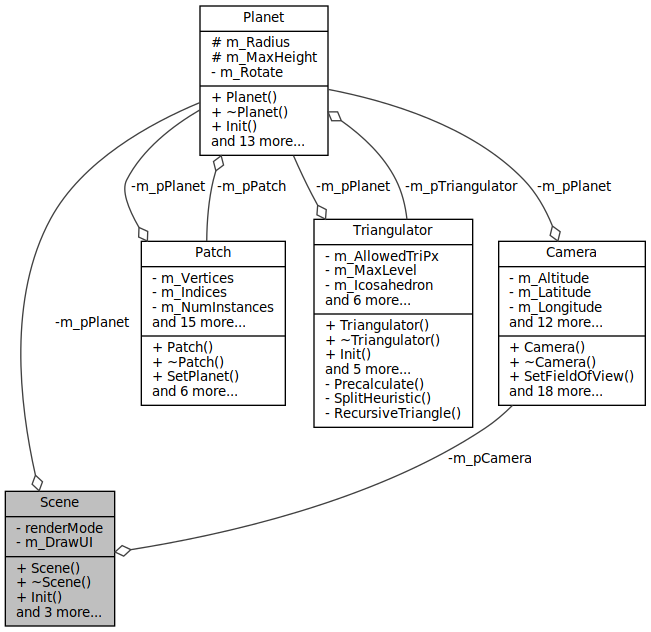
\includegraphics[width=10cm]{img/uml_scene.png}
  \caption{Diagramme de classe de Planet}
  \label{fig:uml_scene}
  \end{figure}

  La classe Scene est la classe centrale du programme, elle permet
  d'initialiser et de créer la planète. Scene gère les paramètres
  principaux du programme à travers les entrées clavier d'InputManager.
  Ces paramètres sont le nombre de niveaux de détail, le mode d'affichage
  (texture + maillage, maillage uniquement, texture uniquement). Scene
  gère aussi l'affichage des informations comme le compteur d'images par
  seconde ou le nombre de sommets actuellement affiché.
  
  La classe Planet représente la sphère à afficher. Ses classes filles
  spécialisent le type de planète à afficher, ce sont elles qui
  définissent la taille de la sphère, sa texture et sa carte de hauteur.\\
  \textbf{graphe d'héritage de Planet quand Procedural sera merge}
  
  %\begin{figure}
  %centering
  %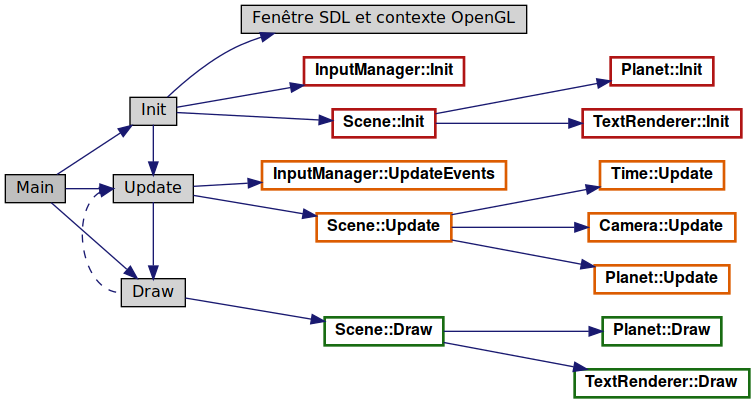
\includegraphics[width=10cm]{img/plan_exec.png}
  %\caption{Plan}
  %\label{fig:triangulator}
  %\end{figure}
 
  La figure \ref{fig:plan} représente le graphe simplifié de
  l'exécution du programme. L'étape d'initialisation se fait une seule
  fois au début du programme, et les étapes de mise à jour et d'affichage
  se répètent tout le long de l'exécution.
  
  \section{Triangulator}
  La classe Triangulator permet de générer le \emph{quadtree} utilisé pour le système de niveau de détail.
  Un objet Frustum est utilisé pour décider si un triangle de l'arbre est ou non dans le cône 
  de vision de la caméra. Le diagramme de classes présenté en figure \ref{fig:plan} présente la classe
  Triangulator. Les différents composants seront analysés plus loin dans le chapitre implémentation.
  
  \section{Patch}
  La classe Patch permet de générer et d'afficher le maillage en y appliquant l'algorithme de morphing.
  Le morphing est ce qui permet d'avoir des transissions douces entre les différents niveaux de détails.
  Les détails seront expliqués plus loin dans la partie implémentation.
  
  
  \begin{figure}
  \centering
  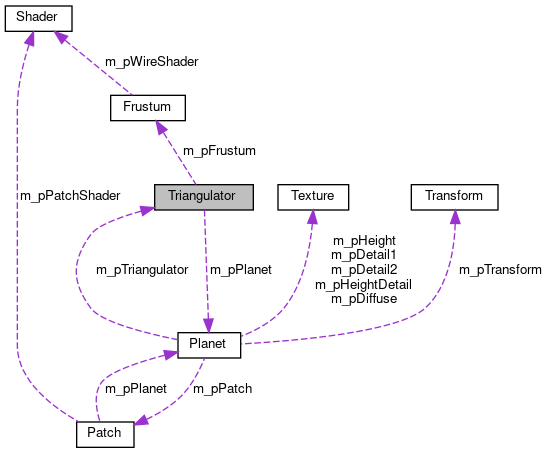
\includegraphics[width=10cm]{img/triangulator.png}
  \caption{Diagramme de classe de Triangulator}
  \label{fig:plan}
  \end{figure}
  
  \section{Frustum}
  La classe Frustum permet de faire des opérations sur les triangles qui sont dans le cône de vision de la caméra. Le Frustum utilisé par la classe Triangulator pour permettre les tests d'union entre les triangles est le cône de vision. La classe Frustum permet aussi de décider si un triangle est à afficher ou non.\\
  
  Cette classe permet entre autres d'éliminer les triangles qui ne sont pas visibles de la caméra. Cette opération appelée \textit{culling} permet d'éviter d'envoyer des triangles inutiles à la carte graphique.
  Dans ce cas ci,-cela permet aussi d'éliminer ces triangles de l'arbre et donc d'optimiser sa génération.
  
 \newpage %pour placer les images correctement
 